\documentclass{article}
\usepackage{graphicx}

\begin{document}

\begin{titlepage}
    \centering
    \vfill
    {\bfseries\Large
        Mistborn Ragnarok - Aggressive Pigeon Studios\\
        Game Design Document\\
        October 31st, 2019\\
        Rev. 4.0\\

        \vskip1cm
        Christian Plourde 26572499\\
		Ayush Kharade 40042388\\
		Daniel Vellucci 27416288\\
		Samer Yazbeck 40049573\\
		Luciano Porchet 40048537\\
    }    
    \vfill
    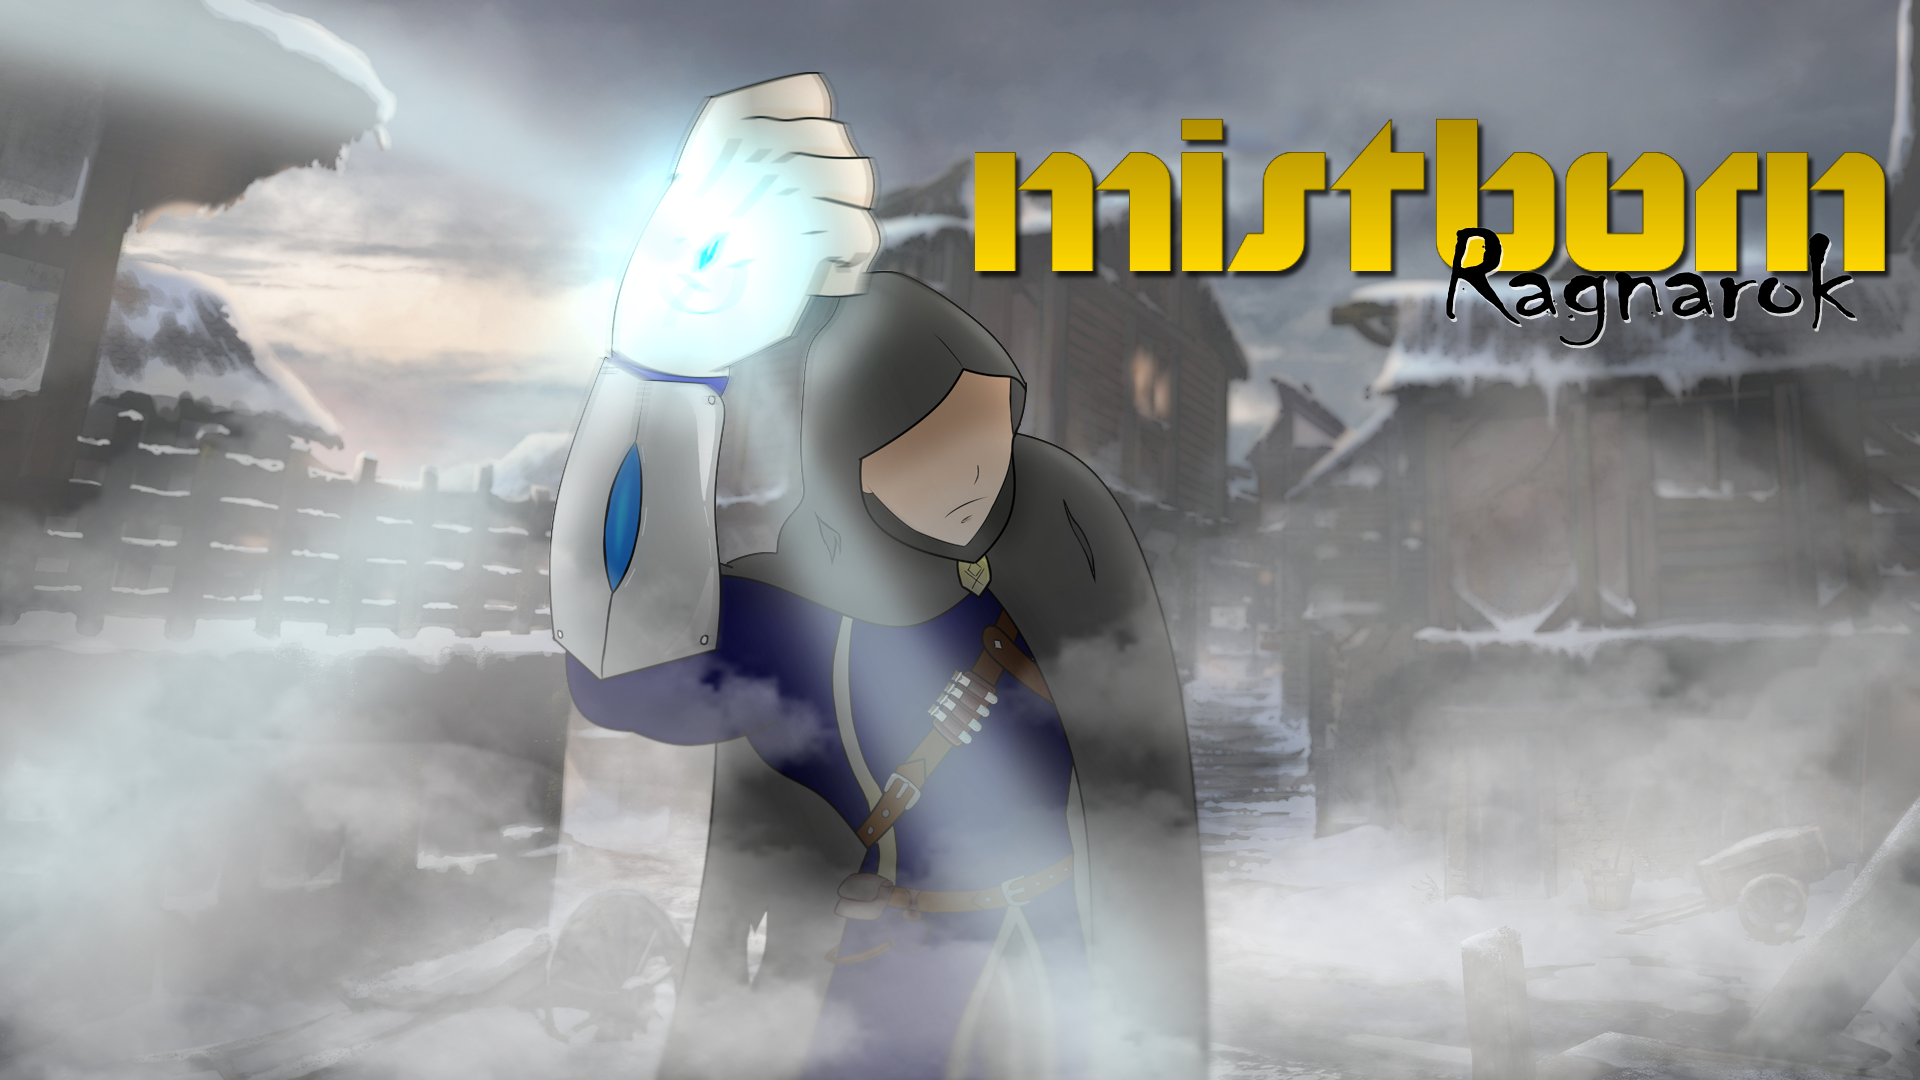
\includegraphics[width=14cm, height=10cm]{Box_Art.png} % also works with logo.pdf
    \vfill
    \vfill
\end{titlepage}

\newpage

\section{Executive Summary}
In an apocalyptic world, follow Jora's quest to find answers as he goes through different obstacles and puzzles. Our game is a fun puzzle platformer with emphasis on the world and its dark setting.

\section{Overview}

Mistborn Rangarok centers around a character who has magical abilities inspired by the Mistborn Series by Brandon Sanderson that allow him to pull and push metals in similar fashion to the Magnesis ability in The Legend of Zelda: Breath of The Wild. This is used to fight enemies and solve puzzles.
\\*\\*
The main character also has the ability to use pewter in order to make him jump further as well as fight enemies and pick up heavy objects. These abilities help him defeat enemies and solve puzzles as well as make platforming jumps that are otherwise impossible.
\\*\\*
Follow Jora's story as you find different notes explaining the lore and the setting. Travel through a dark and immersive world where ash falls constantly from the sky and enemies lurk around every corner. Since the inhabitants of the town seem to have disappeared, Jora finds himself alone on his adventure, lost with no guidance. This ambiance is captured in the lighting and foreboding atmosphere of the game.
\\*\\*
In the first chapter which is a tutorial, the player goes through the city of Luthadel made famous by Brandon Sanderson's novels. The level features enemies and a lot of platforming, as well as traps that the player must avoid. It concludes with a simple puzzle to introduce the player to the mechanics of the game while developing the story.
\\*\\*
The second chapter takes place outside the town, in a forest like setting. The player again goes through a lot of platforming and enemies and is introduced to a new enemy type. The level also features more involved puzzles. 
\\*\\*
The game ends with a boss fight in which the player must battle Ruin, the main villain in the game, in a cave outside the city where lies the Well Of Ascension, an ancient source of power. The player must fight through varying phases and find a way to evade the bosses various attacks in order to defeat him.

\section{Related Games}

\subsection{Hollow Knight}
Hollow Knight is a game developed by Team Cherry and is an Action Platformer PC game released in 2017.
Fight enemies in a forsaken world using spells and abilities unlocked along the way. Platforming areas lead to a final boss fight, requiring the player to use the abilities he/she has learned along the way. Mistborn implements similar mechanics especially abilities to fight enemies, and a boss fight. Hollow Knight has a really dark and gloomy setting which makes it very appealing and fits well with its story. The atmosphere of this game is similar to what we are trying to emulate.

\subsection{INSIDE}
INSIDE is a game developed by Playdead and is an Indie Platformer PC game released in 2016.
The protagonist is being hunted by an entity while everyone else is enthralled by the entity. The protagonist has to sneak around and solve puzzles. This dark setting resembles the mistborn world. It also implements similar puzzle solving mechanics. The best part of INSIDE is its story and how immersive it is. We aim to replicate this in our game, as we want the player to get involved in the story and to be intrigued by the final revelations.

\subsection{Trine}
Trine is a game developed by FronzenByte and is an Action Platformer PC game released in 2009.
Trine is a fantasy setting platformer, where the player fights enemies, solving puzzles along the way. Use character abilities to interact with the environment and achieve you goal. Mistborn is inspired by the puzzle solving element and the ability to interact with the world. Trine has very nice 3D graphics but has 2D side scrolling action which is the style of game we want to use in Mistborn.

\section{Player Composites}

"Alliser thorne, 27, museum guard. Single, Graduate of Loyola College. Plays games alone a couple time a week, and with other members of the museum on his days off. Focuses on competitive, action games like Gears of War and Call of Duty. Watches esports and sometime rides horses at his parents farm."
\begin{description}
	\item When and where does this person play games? On his days off at home on his PC
	\item What platforms does this player use? PC 
	\item How much time does this person spend in each session, and
	how frequent are gaming sessions? Twice to three times a week for 4h each
	\item Who does he or she play with? His coworkers 
	\item What does the player like about games? They are fun and bring out his competitive side
	\item What (non-game) brand images appeal to this player? RedBull
	\item How much disposable income does this player have? 30000\$ a year
	\item What competes with gaming time for this player? He learns Jiu Jitsu.
\end{description}

\section{Game World}
After a brutal attack at sea, Jora, the main character, wakes up after being cast ashore in a small rescue boat to the sights of an abandoned village. The world around him is cold and desolate and ash perpetually falls from the sky, covering the landscape in a black blanket. Due to the Lord Ruler’s influence after seizing the power at the Well of Ascension 1000 years ago, the planet lies dangerously close to the sun – a fiery red ball in the sky. The Well has since been replenished and our protagonist feels it beckoning to him. The traumatic experience of the attack preceding his shipwreck have snapped Jora, awakening the Mistborn powers he was genetically predisposed to. As the prophecies foretold, the Hero of Ages must once again travel to the Well of Ascension and seize its power. What awaits him there will require mastery of his newly acquired powers to overcome and save the world from impending doom.
\\*\\*
 As he travels he will understand more of the world that surrounds him and of the events that have transpired through the story of a Mistborn that came before. Once he arrives at the Well of Ascension he will encounter the god Ruin who appears to have taken a flesh body for the fight. Once you have defeated him Jora will feel relieved knowing that the horror is now over not knowing that Ruin still lives on.

\section{Game Characters}

\subsection{Jora}
The main character of the game, Jora is a Viking from the city of Luthadel. He wears a blue and gold colored robe, with a strap across his chest to hold vials of metals that he can consume to recharge his abilities. On his way back from a trip, something strange happened to him and his crew, leaving him as the only survivor. Equally, Jora starts to hear a strange thumping noise that seems to be drawing him towards something. He decides to follow this thumping, hoping to shed light on what happened to his crew and the inhabitants of the city.

\begin{figure}[!htb]
  \caption {Jora Concept Art}
    \center{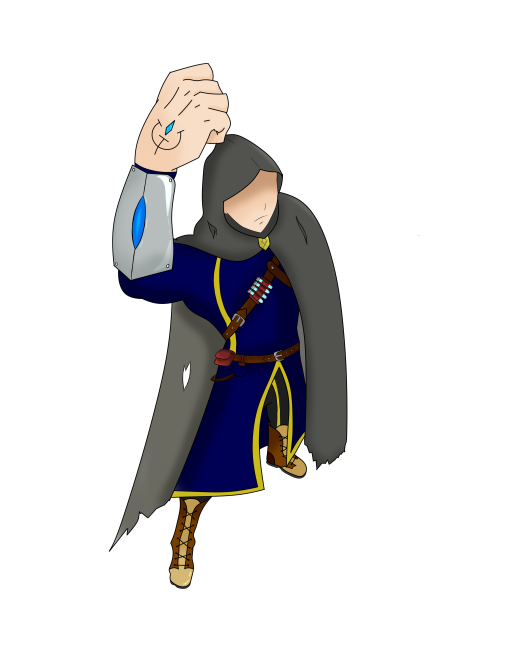
\includegraphics[width=5cm, height=5cm]
    {jora.png}}
  \end{figure}


\subsection{Ruin}
The main antagonist of the game is Ruin. The player encounters him in the final level, which is a boss fight. Ruin is the god of destruction, and plans on destroying the world using the power at the Well of Ascension. Since Ruin cannot access the power directly, he tricks Jora into coming to the Well and taking the power, then giving it up, as is the honorable thing to do. Ruin then plans to take the power and finish off the apocalypse.

\subsection{Kelsier}
Kelsier (known in game as the mysterious K) is the person who has left the lore notes throughout the game.
As a side character you read about through your adventure, the mysterious K is a reference to Kelsier from the original novel. He is there to guide the player throughout the game and bring useful information to the story of the game.
\\*\\*
We don’t know much of K other then like us he is a Mistborn that has been hearing the sounds driving us to go to the Well. But unlike us he is more knowledgeable of the art of being a Mistborn and thus his notes serve to guide the player. Not much else is know about him other than the fact that he most likely died since his last notes leave us with the idea that he was going to fight Ruin.

\section{Art Direction}

Both the game's setting and mechanics are inspired heavily by the Mistborn Trilogy by Brandon Sanderson. Some concept art depicting the game's setting can be seen below.

\begin{figure}[!htb]
  \caption {Crewmate Fighting}
    \center{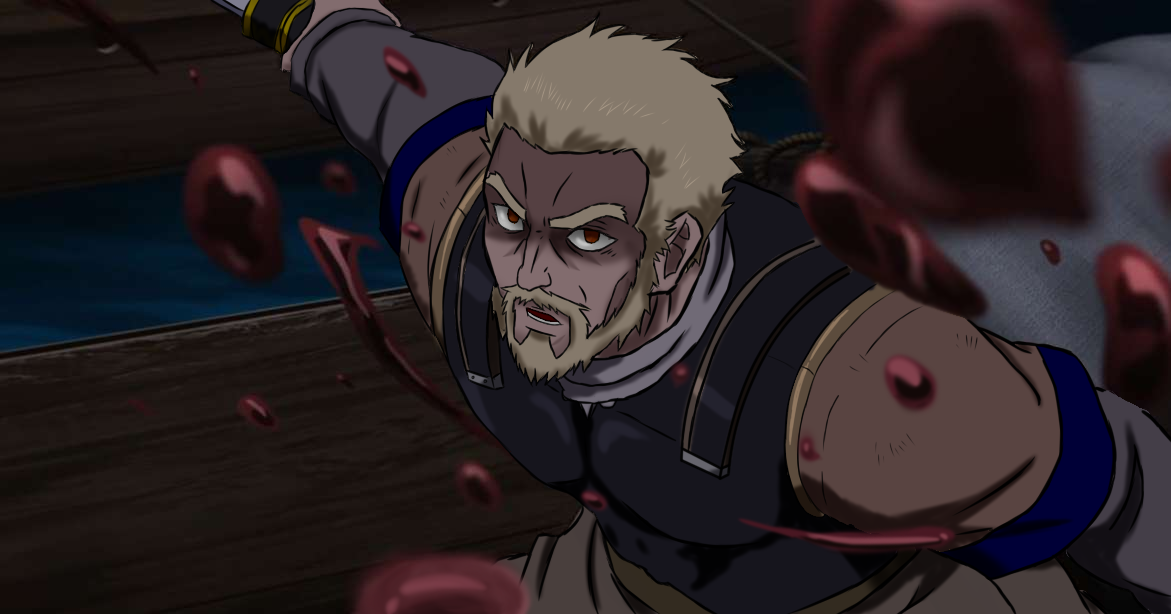
\includegraphics[width=4cm, height=4cm]
    {cutscene_1.png}}
  \end{figure}

  \begin{figure}[!htb]
  \caption {Jora's Loneliness}
    \center{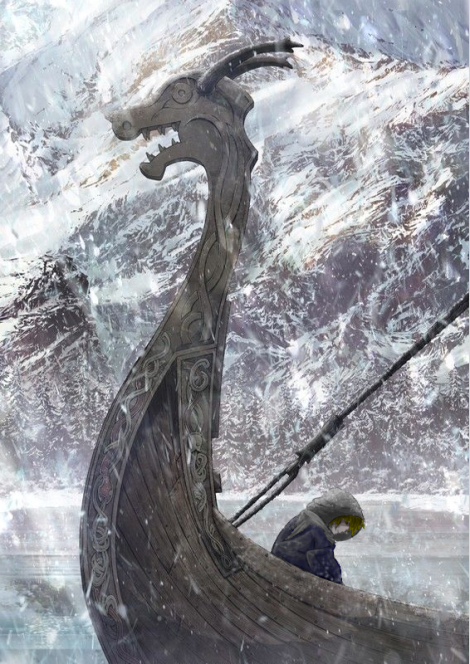
\includegraphics[width=4cm, height=4cm]
    {cutscene_2.png}}
  \end{figure}

  \begin{figure}[!htb]
  \caption {Jora's Determination}
    \center{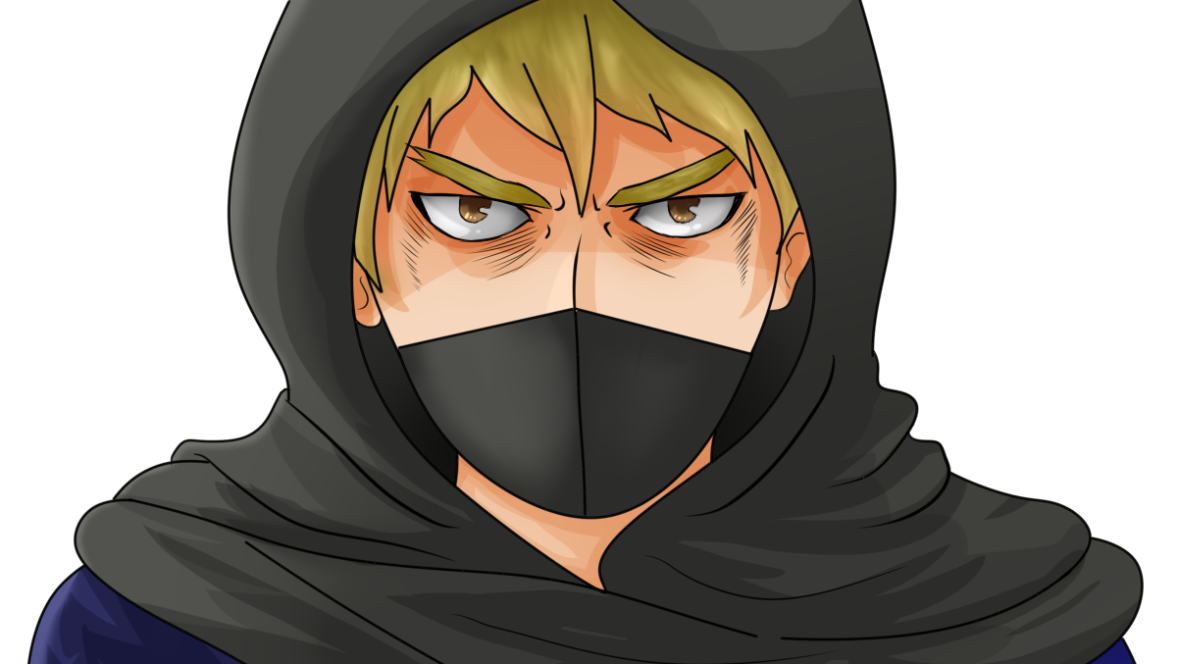
\includegraphics[width=4cm, height=4cm]
    {front_faceshot.png}}
  \end{figure}

\section{User Interface}

The user interface has a health bar depicting the character's remaining health, the potion that he is using as well as a timer bar that shows how much time is left on the active potion. This is placed in the top left corner of the screen.\\

It also has a hotbar that shows a boat with three different icons. These represent the number of potions of each type the player currently has on him. This is found in the middle at the bottom of the screen.

 \begin{figure}[!htb]
  \caption {Screenshot of Game With UI Elements}
    \center{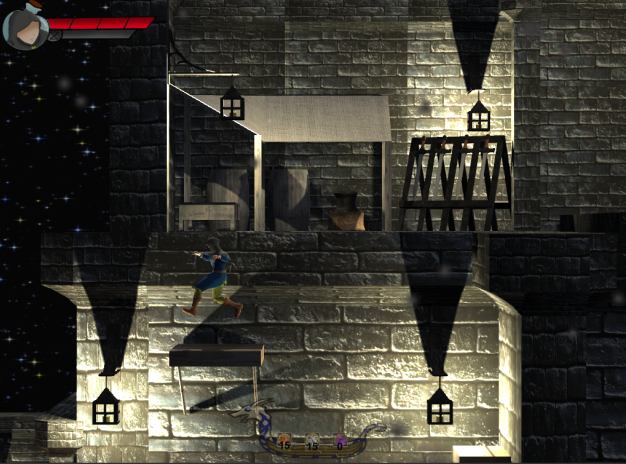
\includegraphics[width=10cm, height=8cm]
    {screenshot.png}}
  \end{figure}

The main menu is accessible from in game and allows the player to pause the game. It contains a button to resume the game as well as to quit and return to the title screen. This title screen is a menu that allows the player to begin playing the game (from level one), quit the application, and play the credits, which will play a small video crediting the makers of the game.

\begin{figure}[!htb]
  \caption {Screenshot of In-Game Menu}
    \center{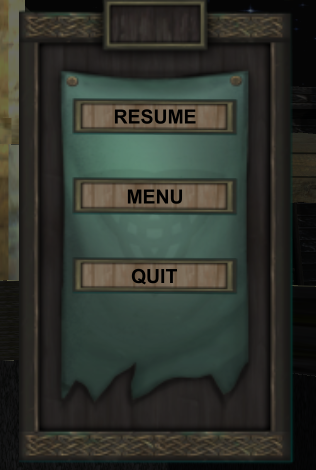
\includegraphics[width=3cm, height=4cm]
    {MainMenu.png}}
  \end{figure}

\section{Technology Plan}
We used blender to make the assets and unity to build and create the game (with unity physics). We also used Autodesk Maya to create the character and all it's associated animations.\\*\\*

For writing the scripts we used Visual Studio. The cutscene art and GUI art were drawn in Painttool Sai. We used Latex to write the GDD and we organized and managed the project with the use of both Discord for communication and GitHub for organization and version control. Finally the first draft of each level design was made in draw.io.

\section{Controls}
The "A" and "D" keys allow the player to move right and left.\\
The "W" and "S" keys allow the player to go up and down ladders.\\
The “Space” key allows the player to jump.\\
The following keys allow the activation of the three potions.
\begin{description}
	\item[1] Iron Potion
	\item[2] Steel Potion
	\item[3] Pewter Potion
\end{description}
Left Clicking allows the player to interact with objects using powers.\\
The "E" key allows the player to interact with objects without powers.\\
The "P" key allows the player to pause the game.\\
The "Esc" key to close notes when they are open.

\section{Level Design}
The level design is linear, while going from the far left side of the level to the far right side, while solving puzzle and overcoming obstacles and enemies. At the end of each level, the player is transported automatically to the next level after a cutscene for a total of two levels and a boss fight.\\

Obstacles include enemies, platforming, traps such as tripwires and spike pits. The puzzles are typically solved by using iron and steel to push or pull objects onto pressure plates, move objects out of the way, or activate levers and trapdoors. Throughout the map, chests can be found and opened containing potions that can be used to solve the puzzles or fight enemies as well as notes explaining the lore of the game.\\

In Level 2, there is a large tower with a complex platforming segment. Right before it, there is another tower with two levels and a roof. If the player goes through the second level, the enemy can be bypassed and the second tower can be platformed to via the roof. However, if the player falls from the first or second tower, the only way to proceed is to go through the enemy. This will force the player to be extra careful in this section since he will have to fight the enemy if he fails the platforming section. This essentially creates an easy path and a difficult path which makes the level design more interesting by presenting the player with options as to where he wishes to go.

\section{Mechanics Analysis}
The game has a total of 3 mechanics used to solve puzzles or fight enemies. These are the three powers (iron, steel, and pewter). Iron and Steel uses Unity's physics engine to pull and push metal objects around. Pewter gives access to fighting to overcome enemies and so does not rely on Unity's physics engine. Since these potions are available in limited supply it is important for the player to manage these resources to be able to progress through the levels.\\

The main way to move about the level is through platforming. This makes progress through otherwise easy sections of the level challenging, requiring precision jumping from the player. Platforming is a very popular mechanic and has made games like Celeste very popular due to its challenging nature.\\

The game also features a total of three puzzles. The puzzles, as mentioned before are classic lock and key puzzles. They are all different but require the player to do a sequence of actions to unlock a pathway through. In the final puzzle, the player must make it through 3 doors, each one being opened in a different way, with the final door being opened with a literal "key" that the player must find.\\

The boss has some unique mechanics and he is divided in two stages. In both stages the window during which you can interact/fight him in is small so you need to dodge using platforming skills until it's time to fight him using one of the potions (depending on the stage). This adds difficulty and is a good way to implement a nice ending to the game.


\section{Project Status}
The tasks/mechanics that have been implemented are:
\begin{description}
	\item Platforming
	\item Ladders
	\item Iron and Steel Abilities
	\item Regular Enemies (Bandits)
	\item Combat with Pushing and Pulling
	\item Pewter Ability
	\item Sound Design
	\item Level 1 Layout
	\item Ranged Enemy
	\item Highlighting Interactables
	\item Boss Fight
	\item Level 2 Layout
	\item Boss Level Layout
	\end{description}

\section{Meeting Durations}
\begin{description}
	\item September 18th 2019 - 90 minutes 
	\item September 25th 2019 - 90 minutes
	\item September 28th 2019 - 90 minutes
	\item October 2nd 2019 - 90 minutes (Dropped combined potions mechanic)
	\item October 9th 2019 - 90 minutes
	\item October 16th 2019 - 90 minutes
	\item October 23rd 2019 - 90 minutes
	\item October 30th 2019 - 120 minutes
	\item November 6th 2019 - 90 minutes
	\item November 13th 2019 - 90 minutes (Koloss enemy type dropped)
	\item November 20th 2019 - 90 minutes (Dropped boss fight's last phase - went from 3 phases to 2 phases)
	\item November 27th 2019 - 90 minutes
	\end{description}

\end{document}